%Para este capítulo se usará la abreviatura "cont".
\chapter{Continuidad}
\label{cont}

La continuidad es la propiedad por excelencia que queremos que nuestras funciones verifiquen. En este breve capítulo vamos a generalizar la noción de continuidad que ya conocemos y dominamos para espacios como $\R^n$, de forma que la podamos aplicar a cualquier espacio topológico conocido (sin necesidad de que sea métrico). La continuidad, además, será clave para definir más adelante la noción de homeomorfismo, es decir, una transformación que preserva las propiedades topológicas de un espacio dado.

\section{Definición y propiedades elementales}

Para empezar, tratamos de dar una justificación intuitiva del cómo se llegó a la definición que presentaremos a continuación.

Hasta ahora conocíamos una definición de continuidad válida en el ámbito de los espacios métricos, que nos decía que si $(M,d)$ y $(N,d')$ eran espacios métricos arbitrarios y $f:M\to\N$ una aplicación entre ellos, era continua en un punto $x_0\in M$ si y solo si dado un $\varepsilon>0$ podíamos encontrar un $\delta>0$ de forma que $f(\bola_d(x_0,\delta))\subset\bola_{d'}(f(x_0),\varepsilon)$.

Dicho de otra forma, si cierto punto dista de $x_0$ menos que $\delta$, entonces su imagen deberá distar menos que $\varepsilon$ de la imagen de $x_0$. Informalmente, una aplicación continua es la que manda puntos próximos a puntos próximos.

En los espacios topológicos no tenemos la noción de distancia, pero si cierta noción de ``proximidad'', o al menos de ``ligadura'' entre puntos, esta es la noción de entorno, que usaremos para extender esta definición.
\begin{defi}[Continuidad en un punto]
	Sean $\X$ e $\Y$ espacios topológicos. Consideremos asimismo una aplicación $f:\X\to\Y$.
	
	Diremos que $f$ es \tbi[aplicación!continua]{continua} en un punto $x_0\in\X$ si para todo entorno $V_{f(x_0)}$ de $f(x_0)$, la imagen inversa de dicho entorno, $f^{-1}(V_{f(x_0)})$, es entorno de $x_0$. 
\end{defi}

Dicho con palabras llanas, $f$ es continua en un punto si transforma entornos en entornos por imágenes inversas.

Una forma totalmente equivalente de entender este concepto es pensar que dado un entorno $V_{f(x_0)}$ de $f(x_0)$ siempre podremos encontrar un entorno $V_{x_0}$ de forma que $f(V_{x_0})\subset V_{f(x_0)}$.
\begin{obs}[Importancia de las topologías]
	\label{cont_obs_importanciaTopol}
	Si la topología de $\X$ es fina (con muchos abiertos), o la topología de $\Y$ es muy grosera (con muy pocos abiertos), la continuidad suele ser más fácil de comprobar, ya que hay pocos entornos que chequear en el espacio de llegada y muchos candidatos en el espacio de partida.
\end{obs}
Al hilo de la observación \ref{cont_obs_importanciaTopol} veamos algunos casos extremos que pueden resultar chocantes para una mente poco experimentada en los exóticos placeres topológicos.
\begin{obs}[Casos extremos]
	\label{cont_obs_continuidad_discreta_trivial}
	Veamos cual es el comportamiento de la continuidad con las topologías más drásticas que conocemos.	
	\begin{enumerate}
		\item En la topología discreta, cualquier conjunto es abierto, con lo cual $\{x_0\}$ es abierto y, por tanto, cualquier conjunto que contenga a $x_0$ es entorno suyo. Entonces, para cualquier entorno de $f(x_0)$ su imagen inversa contendrá a $x_0$ y por lo anterior será entorno suyo. Es decir, cualquier función que nazca en $\X$ con la topología discreta es continua.
		
		\item En la topología trivial, los únicos abiertos son el vacío y el total, con lo cual dado un punto, su único entorno es el total. Entonces, si $\Y$ con la topología trivial es el espacio de llegada de una función $f$, $f$ es continua, pues la imagen inversa del total es el total, y este es abierto (y por tanto entorno) en cualquier topología. \qedhere 
	\end{enumerate}
\end{obs}

De la misma forma que podemos estudiar la continuidad para unas ciertas topologías concretas, podemos estudiarla para algunas funciones concretas sin limitarnos a una topología particular. En particular, nos van a interesar la función constante y la función identidad.

\begin{obs}[Aplicaciones constante e identidad] \
	\label{cont_obs_continuidad_cte_e_id}
	\begin{enumerate}
		\item Si $f:\X\to\mc{Y}$ es la aplicación constante $f\equiv b$, entonces $f$ es continua con cualquier topología. En efecto, la imagen inversa de cualquier subconjunto (y en particular de cualquier entorno) de $\mc{Y}$ que contenga a $b$ es el total, que es entorno de todos los puntos (por ser abierto).
		
		\item La continuidad de la aplicación identidad depende de los espacios topológicos sobre los que está definida, al contrario de lo que pueda parecer. Caso curioso es el siguiente:
		\[\text{id}:(\X,\T_\text{discreta})\to (\X,\T_\text{trivial})\]
		Esta aplicación es continua (y biyectiva), por la observación \ref{cont_obs_continuidad_discreta_trivial}. Sin embargo, su inversa, que también es la aplicación identidad, no es continua. Esto se sigue directamente de que, por ser la topología del espacio de llegada la discreta, $\{f(x_0)\}$ es abierto y por tanto entorno de $f(x_0)$, pero su imagen inversa es $\{x_0\}$ que con la topología trivial del espacio de salida no es entorno. \qedhere
	\end{enumerate}
\end{obs}

Ahora, veremos un par de propiedades interesantes de la continuidad en un punto.

\begin{prop}[Continuidad y restricciones]
	Dada $f:\X\to\mc{Y}$, continua en $x_0\in\X$, si $A\subset\X$ tal que $x_0\in A$, entonces $f\restriction_A:A\to\mc{Y}$ es continua en $x_0$.
	
	\begin{proof}
		Sea $V_{f(x_0)}$ un entorno de $f(x_0)$. Se verifica que $(f\restriction_A^{-1})(V_{f(x_0)}) = A\cap f^{-1}(V_{f(x_0)})$. Pero como por la continuidad de $f$ en $x_0$ tenemos que $f^{-1}(V_{f(x_0)})$ es entorno de $x_0$ en $\X$, entonces $A\cap f^{-1}(V_{f(x_0)})$ es entorno de $x_0$ en $A$ (nótese que consideramos la topología relativa en $A$).
	\end{proof}
\end{prop}

	Este lema viene a decirnos que la continuidad no depende del conjunto donde nos encontremos, no obstante, si depende (y mucho) de la topología.
	
	La siguiente proposición es el recíproco de la anterior.

\begin{prop}[Continuidad como propiedad local] Si hay un entorno $V_{x_0}$ de $x_0$ tal que $f\restriction_{V_{x_0}}$ es continua en $x_0$ entonces $f$ es continua.
	
	\begin{proof}
		Sea $V_{f(x_0)}$ un entorno de $f(x_0)$, por continuidad de  $f\restriction_{V_{x_0}}$ en $x_0$ se cumple que $(f\restriction_{V_{x_0}})^{-1}(V_{f(x_0)}) = f^{-1}(V_{f(x_0)})\cap V_{x_0}$ es entorno de $x_0$ en $V_{x_0}$, luego, por topología relativa, $f^{-1}(V_{f(x_0)})$ es entorno de $x_0$ en $\X$ y, por tanto, $f$ es continua.
	\end{proof}
\end{prop}

	La idea que define a las llamadas ``propiedades locales'', es que para ver si se cumplen en un punto no es necesario mirar como se comporta todo el espacio en su conjunto, sino tan solo debemos comprobar como se comporta en un entorno del punto.
	
	La idea intuitiva de esto es que nos da igual lo que pase ``lejos'' del punto.

\section{Caracterizaciones de la continuidad}

Tras definir la continuidad en un punto, el paso instintivo es por supuesto definir la continuidad en todo el espacio (o en cualquiera de sus subconjuntos). Vamos a hacerlo y a dar una serie de definiciones equivalentes de continuidad, que abren muchas posibilidades a la hora de verificar esta propiedad.

\begin{defi}[Continuidad en un conjunto]
	Se dice que $f:\X\to\mc{Y}$ es \tbi[aplicación!continua]{continua} en un conjunto $A\subset \X$ si lo es en todo punto de $A$.
\end{defi}

Vamos a ver ahora una serie de definiciones equivalentes de la noción de continuidad.

\begin{prop}[Caracterizaciones de la continuidad]
	\label{cont_prop_caracterizacion}
	Sea $f:\X\to\mc{Y}$. Entonces, las siguientes afirmaciones son equivalentes:
	
	\begin{enumerate}
		\setcounter{enumi}{-1}
		\item $f$ es continua
		\item La imagen inversa de cualquier abierto es abierta.
		\item La imagen inversa de cualquier cerrado es cerrada.
		\item $f(\adher{A})\subset\adher{f(A)}$ para cualquier subconjunto $A$ de $\X$.
		\item Existe un recubrimiento abierto arbitrario de $\X$ de la forma:
			\[\X=\bigcup\limits_{i\in I} U_i\]
			que verifica que todas las restricciones $f\restriction_{U_i}$ son continuas.
		\item Existe un recubrimiento cerrado finito de $\X$ de la forma:
			\[\X=\bigcup\limits_{i=1}^k F_i\]
			que verifica que todas las restricciones $f\restriction_{F_i}$ son continuas.
	\end{enumerate}

	\begin{proof}
		Procederemos según el siguiente diagrama, no obstante, se reta al lector a tratar de efectuar cualquiera de las implicaciones no demostradas explícitamente.
		\[
		\xymatrix{&(0.)\ar@2{<->}[r]\ar@{=>}[d]&(1.)\ar@2{<->}[dr]& &\\
			&(4.)\ar@{=>}[ur] & &(2.)\ar@2{<->}[r]&(3.)\\
			(5.)\ar@{<=}[uur] \ar@{=>}[urrr]& & & &}
		\]
		\begin{enumerate}[align=left, leftmargin=*]
			\item[\fbox{$(0)\implies (1)$}] Sea un abierto $U\subset\mc{Y}$. Por ser abierto, es entorno de todos sus puntos. Pero para cada punto $f(x_0)\in U$, por ser $f$ continua, la imagen inversa de $U$ es también entorno de $x_0$. De esta forma, para cualquier $x_0\in f^{-1}(U)$, se cumple que $f^{-1}(U)$ es entorno de $x_0$, y por tanto $f^{-1}(U)$ es abierto.
			
			\item[\fbox{$(1)\implies (0)$}] Sea $V_{f(x_0)}$ un entorno en $\mc{Y}$. Por definición, contiene un abierto $U$ tal que $f(x_0)\in U$. Ahora, por hipótesis, $f^{-1}(U)$ es abierto, y como $x_0\in f^{-1}(U)\subset f^{-1}(V_{f(x_0)})$, se verifica que $f^{-1}(V_{f(x_0)})$ contiene un abierto que contiene a $x_0$ y por tanto es entorno.
			
			\item[\fbox{$(1)\Longleftrightarrow (2)$}] $F\subset\mc{Y}$ es cerrado si y solo si $\mc{Y}\setminus F$ es abierto. Pero entonces por hipótesis $f^{-1}(\mc{Y}\setminus F)$ es abierto, y $f^{-1}(\mc{Y}\setminus F)=\X\setminus f^{-1}(F)$, luego $f^{-1}(F)$ es cerrado. La otra implicación es análoga.
			
			\item[\fbox{$(2)\implies (3)$}] Basta con ver que cualquier $A$ verifica que $f(\adher{A})\subset \adher{f(A)}$ o, lo que es equivalente, $\adher{A}\subset f^{-1}(\adher{f(A)})$. Sin embargo, la imagen inversa del cerrado $\adher{f(A)}$ es cerrada, con lo que basta con demostrar que $A\subset f^{-1}(\adher{f(A)})$, ya que $\adher{A}$ es el menor cerrado que contiene a $A$. Por tanto, simplemente:
			\[A\subset f^{-1}(f(A))\subset f^{-1}(\adher{f(A)})\]
			porque $f(A)\subset\adher{f(A)}$.
			
			\item[\fbox{$(3)\implies (2)$}] Sea $F\subset\mc{Y}$ cerrado. Queremos probar que $G=f^{-1}(F)$ también lo es, y tenemos, por hipótesis y por las propiedades de la imagen inversa:
			\[f(\adher{G})\subset\adher{f(G)}=\adher{f(f^{-1}(F))}\subset\adher{F}=F\]
			pero entonces $\adher{G}\subset f^{-1}(F)=G$, luego $\adher{G}=G$ y entonces $G$ es cerrado por la proposición \ref{etop_prop_cerradosAdher}.
						
			\item[\fbox{$(0)\implies (4)$}] Trivial, con el recubrimiento cuyo único abierto es $\mc{X}$.
			
			\item[\fbox{$(4)\implies (1)$}] Vamos a aprovechar que ya hemos demostrado $(0)\iff (1)$. Entonces, sea $U\subset\mc{Y}$ un abierto. Lo podemos escribir como unión de abiertos de forma que cada uno de ellos esté en un $U_i$, de la siguiente forma:
			\[U=\bigcup\limits_{i\in I} (U_i\cap U)\]
			
			Ahora, la imagen inversa de $U$ es:
			\[f^{-1}(U)=f^{-1}\left(\bigcup\limits_{i\in I} (U_i\cap U)\right)=\bigcup\limits_{i\in I} (f^{-1}(U_i\cap U))\]
			pero como $U_i\cap U\subset U_i$ y $f\restriction_{U_i}$ es continua, entonces cada una de estas imágenes inversas es abierta, luego la imagen inversa de $U$ también lo es por ser unión arbitraria de abiertos.
			
			\item[\fbox{$(0)\implies (5)$}] Trivial, con el recubrimiento cuyo único cerrado es $\mc{X}$.
			
			\item[\fbox{$(5)\implies (2)$}] Es análogo a $(4)\implies (1)$. \qedhere
		\end{enumerate}
	\end{proof}
\end{prop}

Terminamos con una propiedad fundamental de las funciones continuas, y es que la composición respeta la continuidad.

\begin{prop}[Composición]
	Sean $f:\X\to\mc{Y}$, $g:\mc{Y}\to\mc{Z}$, con $f,g$ continuas. Entonces, $h = g\circ f$ es continua.
	
	\begin{proof}
		Esta es una consecuencia casi directa de la definición. En efecto, si consideramos $x_0\in\X$ y sus imágenes:
		\[x_0\mapsto f(x_0)\eqqcolon y_0\mapsto g(f(x_0))=g(y_0)\eqqcolon z_0\]
		entonces basta con estudiar los entornos. En efecto, si $V_{z_0}$ es entorno de $z_0$, por la continuidad de $g$ su imagen inversa es un entorno $V_{y_0}$ en $\mc{Y}$ y, ahora, por la continuidad de $f$, la imagen inversa de este último es un entorno de $x_0$.
	\end{proof}
\end{prop}
Ahora que ya sabemos un poco más, a modo de satisfacción personal, para que veamos que las matemáticas funcionan, vamos a deducir condiciones necesarias y suficientes para que la aplicación identidad entre dos espacios topológicos sea continua.
\begin{obs}[Aplicación identidad]
	\label{cont_obs_identidad}
	Sean $(\X,\T_1)$ y $(\X,\T_2)$ espacios topológicos y la aplicación identidad entre ellos. Sabemos que $\text{id}$ es continua si y solo si transforma abiertos en abiertos por imágenes inversas. Luego si $\U$ es abierto en $\T_2$, $\text{id}^{-1}(\U)=\U$ debe ser abierto en $\T_1$. Dicho de otra forma, $\text{id}$ es continua si y solo si $\T_2\subset\T_1$.
\end{obs}
\section{Homeomorfismos y homeomorfismos locales}
\label{cont_homeomorfismos}
Intuitivamente, una aplicación continua es la que no ``rompe'' el espacio. Nos permite deformar, aplastar, girar... pero no cortar o pegar. No obstante en esta sección estudiaremos las aplicaciones que no solo ``no rompen'' el espacio, sino que también son en cierto sentido ``reversibles'', estas serán los llamados ``homeomorfismos''.

A bote pronto los homeomorfismos son las aplicaciones que preservan la estructura topológica, es decir los abiertos (véase la proposición \ref{cont_prop_caracterizacion}) del mismo modo que los isomorfismos de grupos preservaban las operaciones.
\begin{defi}[Homeomorfismo]
	\label{cont_def_homeomorfismo}
	Un \tbi{homeomorfismo} entre espacios topológicos $f\colon \X\rightarrow \Y$ es una biyección continua con inversa continua.
	
	Si existe un homeomorfismo entre dos espacios $\X$ e $\Y$ se dice que estos son \tbi{homeomorfos}.
\end{defi}

Hagamos ahora una pequeña observación antes de pasar a una serie de ejemplos que nos permitan asentar estos conceptos.

\begin{obs}[Continuidad de la inversa]
	\label{cont_obs_defHomeomorfismo}
	Como vemos en la definición \ref{cont_def_homeomorfismo}, no nos basta únicamente con que nuestra aplicación $f$ sea biyectiva (y de este modo tenga inversa) y continua, sino que además exigimos esta inversa sea continua. 
	
	Nótese que, por ejemplo, en los isomorfismos de grupos, siempre que teníamos un homomorfismo biyectivo automáticamente era un isomorfismo. Esto no ocurre en este contexto como veremos a continuación.
	
	Esta continuidad en ambos sentidos del homeomorfismo nos va a resultar muy útil como veremos más adelante, dado que las muchas propiedades (abiertos, cerrados\dots) se van a transladar entre los dos espacios homeomorfos que nos proporciona $f$.
\end{obs}

Ahora pasamos a observar una serie de funciones homeomorfas y no homeomorfas, para comprender las diferencias entre ambas y así afianzar la definición.
\label{etop_exa_homeomorfismos}
\begin{exa}[Homeomorfismos] Comencemos volviendo al ejemplo recurrente de la aplicación identidad.
	\begin{enumerate}
		\item La función $\text{id}\colon(X,\T_{\text{dis}})\rightarrow(X,\T_\text{triv})$ verifica ser continua y biyectiva, pero como vimos en la observación \ref{cont_obs_identidad} su inversa no es continua, por lo que no es un homeomorfismo. 
		
		\item Cualquier función $f$ que mande $\R$ a la \tbi{lemniscata} $\mc{L}\subset\R^2$ (con la topología relativa) no es homeomorfismo, a pesar de que $f$ pudiera llegar a ser biyectiva y continua.
		
		La lemniscata viene descrita por la imagen de la siguiente función.
		\[\varphi(t):=\left(\frac{t}{1+t^4},\frac{t^3}{1+t^4}\right)\]
		Esto no podemos afirmarlo con nuestros conocimientos actuales, no obstante daremos una demostración intuitiva (ver ilustración \ref{cont_img_lemins}) que no pretende ser formal sino tan solo aumentar el interés del lector.
		
		La justificación sería la siguiente. Dado el punto $O:=(0,0)$ tenemos que:
		\begin{itemize}
			\item Todo entorno pinchado de $O$ tiene cuatro ``componentes conexas'' (sean lo que sean).
			\item Todo entorno pinchado de $f^{-1}(O)$ tiene dos componentes conexas.
		\end{itemize}
		
		Por lo tanto, al no mantenerse la cantidad de componentes conexas entre $X$ e $Y$ se verifica que $f$ no es homeomorfismo (ya veremos por qué).
		\begin{figure}[h!]
			\centering
			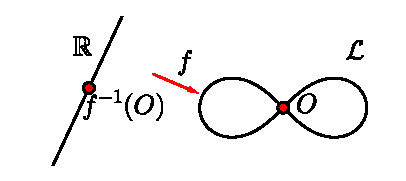
\includegraphics[scale = 0.75]{img/lemniscata}
			\caption{Ilustración del argumento intuitivo.}
			\label{cont_img_lemins}
		\end{figure}
		
		\item \begin{figure}[h!]
			\centering
			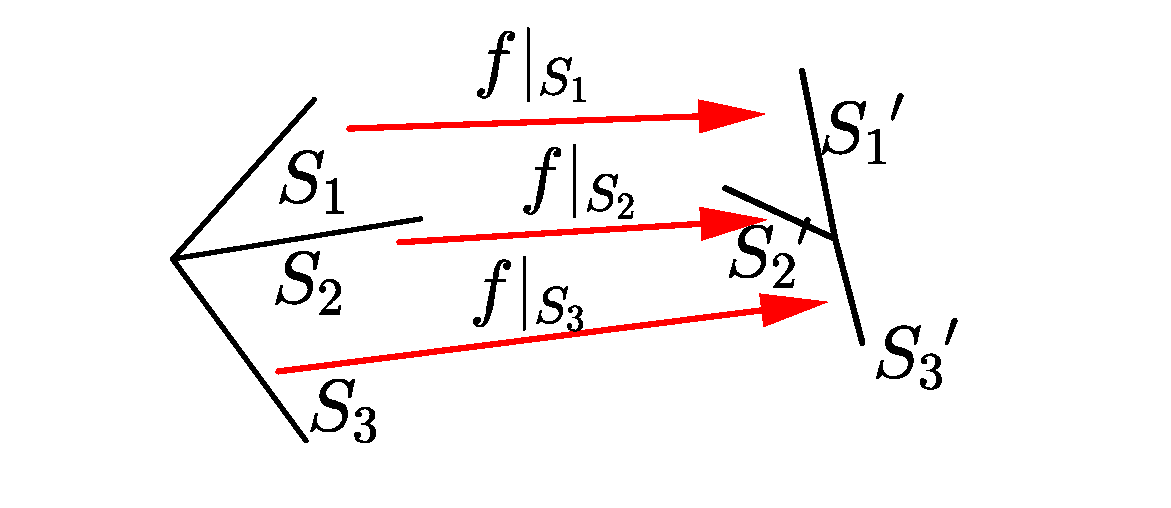
\includegraphics[scale = 0.3]{img/segmentos}
			\caption{Ilustración del homeomorfismo.}
			\label{cont_img_sementos}
		\end{figure}
		
		Sea $\X$ un conjunto $3$ segmentos cualesquiera de $\R^2$ que comparten un punto extremo e $\Y$ otro conjunto de $3$ segmentos arbitrarios que comparten un punto extremo (véase la ilustración \ref{cont_img_sementos}). Si equipamos a ambos conjuntos con la topología relativa inducida por la topología usual de $\R^2$, ambos espacios son homeomorfos.
		
		En efecto, tomando el recubrimiento por cerrados de $\X$ compuesto por cada uno de los segmentos y definiendo un homeomorfismo $f$ que a cada segmento (cerrado del recubrimiento de $\X$) le haga corresponder otro segmento de $\Y$ (sin repetir). Tenemos, por la proposición \ref{cont_prop_caracterizacion} que $\X$ e $\Y$ son homeomorfos (así de paso vemos que las proposiciones sirven para algo).
		
		Dicho homeomorfismo $f$ será la \tbi{interpolación lineal} que definimos como
		\begin{equation}
			\begin{array}{cc}
			f_{ab}:&[0,1]\to\R^2\\
			& t\mapsto ta+(1-t)b
			\end{array}
		\end{equation}
		Que es un homeomorfismo (¡compruébese!) que transforma el intervalo $[0,1]$ en el segmento de $\R^2$ determinado por los puntos $a,b\in\R^2$, al que denotamos por $[a,b]$ con cierto abuso de notación.
		
		Para conseguir un homeomorfismo entre dos segmentos $[a,b]$ y $[c,d]$ cualesquiera basta seguir el siguiente diagrama.
		\[\xymatrix{[0,1]\ar[r]^{f_{ab}}\ar[d]_{f_{cd}}&[a,b]\\
			[c,d]\ar[ru]_{f_{ab}\circ f^{-1}_{cd}}
			}\]
	\end{enumerate}
	Con esto ya tenemos suficiente artillería para resolver gran cantidad de problemas.
\end{exa}

Una vez definido el concepto de homeomorfismo y vista a través de los ejemplos su gran fuerza, vamos a pasar al concepto de homeomorfismo local, el cual, a pesar de ser una relación más débil que la que proporciona el homeomorfismo, también será muy utilizado.

\begin{defi}[Homeomorfismo local]
	\label{cont_def_homeomorfismoLocal}
	Sea $f:X\rightarrow Y$ aplicación entre espacios topológicos y $x_0\in X$. Se dice que $f$ es \tbi[homeomorfismo!local]{homeomorfismo local} en $x_0$ si $x_0$ tiene un entorno abierto $U_{x_0}$ tal que $f(U_{x_0})$ es entorno abierto de $f(x_0)$ en $Y$ y se tiene que $f|_{U_{x_0}}:U_{x_0}\rightarrow f(U_{x_0})$ es homeomorfismo.
\end{defi}

De esta definición se desprende que todo un homeomorfismo entre dos espacios es en un homeomorfismo local en todos sus puntos. Este resultado resulta evidente, pero su contrarreciproco (no homeomorfo local implica no homeomorfo) nos puede resultar enormemente útil ya que es mucho más sencillo estudiar  el homeomorfismo local al global.

Vemos ahora, a modo de ejemplo que la esfera $\esfera^2:=\{x\in\R^3\midc\norm{x}=1\}$ es localmente homeomorfa al plano $\R^2$.

\begin{exa}[Esfera y plano]
	\label{cont_exa_homeomorfismoLocal}
	Vamos a contruir un homeomorfismo local entre la esfera y el plano.
	
	Resulta de interés destacar que no es necesario que la aplicación sea la misma en todo el espacio, sino que podemos tomar una distinta para cada punto del espacio.
	
	En efecto, sea $p:=(x_0,y_0,z_0)\in\esfera^2$ con $z_0\not=0$, entonces, dado un entorno abierto de $p$ que no corta al ecuador de la esfera y queda contenido en el hemisferio de $p$, definimos la aplicación
	\[\begin{array}{cc}
	f(x,y,z):=(x,y) \qquad& f^{-1}(x,y):=(x,y,\frac{z_0}{\abs{z_0}}\sqrt{1-x^2-y^2})
	\end{array}\]
	que es homeomorfismo local (¡compruébese!).
	
	Análogamente, si tomamos un $p':=(x_1,y_1,0)\in\esfera^2$ con $x_1>0$, dado un entorno abierto de $p'$ con todos los puntos con primera coordenada positiva definimos el siguiente homeomorfismo local (¡compruébese!)
	\[\begin{array}{cc}
	f(x,y,z):=(y,z) \qquad& f^{-1}(y,z):=(\sqrt{1-y^2-z^2},y,z)
	\end{array}\]
	Nótese que aún quedan puntos de la esfera por tratar (se dejan como ejercicio).
\end{exa}

Una vez vistas ambas definiciones pasamos a ver una serie de propiedades y observaciones propias de los homeomorfismos (globales), pero que también nos valdrán para la restricción homeomorfa de los locales (dado que en ella por definición la aplicación es homeomorfa).
\label{etop_obs_homeomorfismo}
\begin{obs}[Propiedades de los homeomorfismos]\
	\begin{enumerate}
		\item 
		Sea $f:X\rightarrow Y$ aplicación biyectiva.
		
		Que $f$ sea continua es equivalente a que si $U\in Y$ es abierto, $f^{-1}(U)$ también lo será. Del mismo modo, es equivalente a que si $F\in Y$ es cerrado, $f^{-1}(F)$ también lo será.
		
		Igualmente, que $f^{-1}$ sea continua es equivalente a que si $F\in X$ es cerrado, entonces $f(F)$ es cerrado, asimismo si $U\in X$ es abierto, $f(U)$ también lo será.
		
		Vemos como si se verifican ambas (la continuidad de $f$ y de su inversa) será homeomorfismo, de modo que $f$ es homeomorfismo si y solo si es continua, biyectiva y transforma abiertos en abiertos por imágenes directas.
		
		\item
		Una aplicación $f$ no necesariamente biyectiva se dice \tbi[aplicación!abierta]{abierta} cuando la imagen de abiertos es un abierto (es decir, cuando $f(U)$ es abierta si $U$ es abierto).
		
		Análogamente, una aplicación $f$ no necesariamente biyectiva se llama \tbi[aplicación!cerrada]{cerrada} cuando la imagen de cerrados es un cerrado (es decir, cuando $f(F)$ es cerrado si $F$ es cerrado).
		
		Dejamos como ejercicio al lector ver que si una es aplicación es abierta no tiene por qué ser cerrada (y viceversa) y que si una aplicación es abierta y cerrada no tiene por qué ser biyectiva.\qedhere
		\end{enumerate}
\end{obs}
